\documentclass{article}
\usepackage{graphicx} % Required for inserting images
\usepackage{geometry}
\usepackage[font=small,labelfont=bf]{caption}
\usepackage{subcaption}
\usepackage{float}
%\usepackage{titlesec}
\usepackage[hidelinks, colorlinks=true, allcolors=blue]{hyperref}
\usepackage[french]{babel}
\addto\captionsfrench{\def\tablename{Tableau}}
\usepackage{breqn} % for dmath
\usepackage{siunitx}
\usepackage[T1]{fontenc}
\usepackage{listings}
\usepackage{cleveref}

\geometry{a4paper, margin=2cm}

\edef\restoreparindent{\parindent=\the\parindent\relax}
\usepackage{parskip}

\title{\textbf{TP 3 : Interféromètre de Michelson}}
\author{Pauline Toutain, Hervé Schmit-Veiler}
\date{Avril 2024}


\begin{document}

\maketitle

\section{Introduction}

L'interféromètre de Michelson est un montage expérimental permettant de créer des interférences 
par division d'amplitude.

\begin{figure}[H]
    \centering
    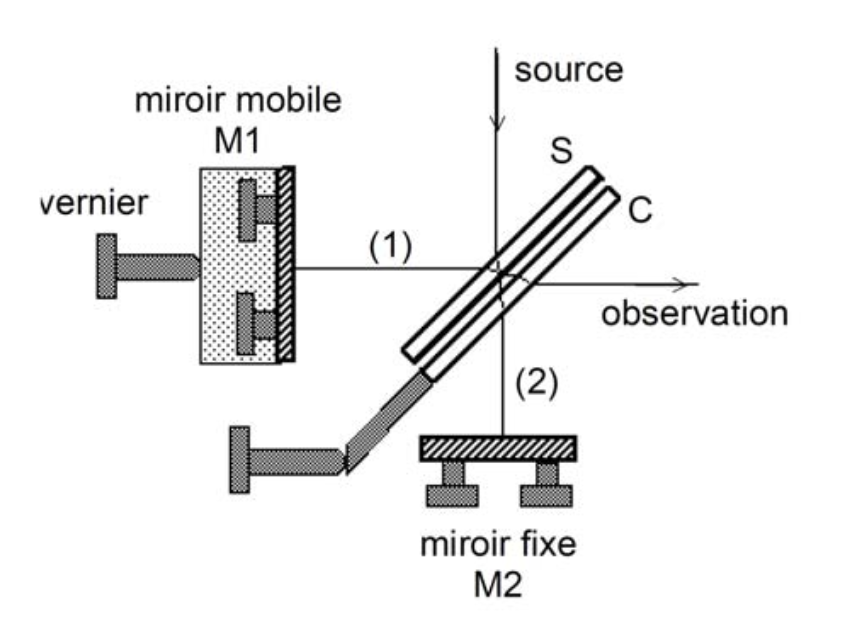
\includegraphics[width=0.5\linewidth]{figs/michelson.png}
    \caption{Schema de l'interféromètre de Michelson provenant du fascicule de TP}
    \label{fig:michelson}
\end{figure}

% Comme indiqué dans le schéma fig. \ref{fig:michelson}, l'amplitude de la source est divisé 
% entre les deux bras de l'interféromètre par une séparatrice semi-réfléchissante S. 
% Au bout des deux bras, se trouvent deux mirroirs M1, M2 qui réfléchissent la lumière vers l'observateur. 
% Dû au longeurs des deux bras différents, les deux rayons (1) et (2) sont déphasés et interfèrent en sortie 
% de l'interféromètre, créant des 

Dans ce rapport, nous présenterons un brève étude de l'interféromètre de Michelson pour la configuration 
"lame d'air". Dans la prémière partie, nous allons d'abord explorer le réglage de l'interféromètre en configuration "lame d'air" ainsi qu'analyser
les figures d'interférences produites par une source étendue. Puis, dans la seconde partie, nous 
utiliserons l'interféromètre pour mesurer l'écart du doublet du sodium, démontrant ainsi la sensibilité et 
la précision de cet instrument. 

\section{Principe de l'interféromètre de Michelson}

Le but de cette première expérience est d'étudier le réglage de l'interféromètre de Michelson 
en configuration "lame d'air", ainsi que d'analyser la figure d'interférences crée à partir d'une source étendue 
– ici une lampe spectrale à vapeur de mercure. 

\subsection{Réglage de l'interféromètre}

% Afin de calibrer le positionnement de la lame semi-réfléchissante, 
% nous avons (avec l'intervention de la professeure) utilisé un laser (source de lumière collimé et monochromatique)

On souhaite manipuler l'interféromètre en configuration "lame d'air", il nous faut donc d'abord régler 
les deux miroirs M1 et M2 parallèls l'un à l'autre.

On place d'abord une lentille de courte focale (un condenseur) après la source afin d'illuminer au plus possible 
le miroir M2 avec de la lumière convergente.

Nous plaçons ensuite un écran diffusant devant la source, ce qui nous permet de calibrer en 
toute sécurité l'interféromètre à l'œil nu. On utilise une croix marquée sur cet écran diffusant 
pour nous guider dans nos réglages.

\begin{figure}
    \centering
    \begin{subfigure}[b]{0.8\textwidth}
        \begin{subfigure}[b]{0.45\textwidth}
            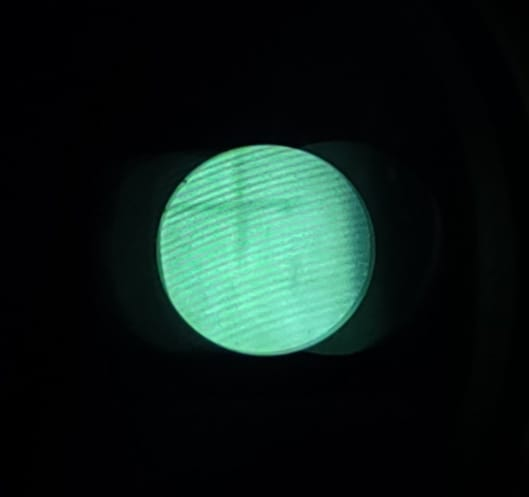
\includegraphics[height=5cm]{figs/croix.jpeg}
            \caption{}\label{fig:croix}
        \end{subfigure}
        \hfill
        \begin{subfigure}[b]{0.45\textwidth}
            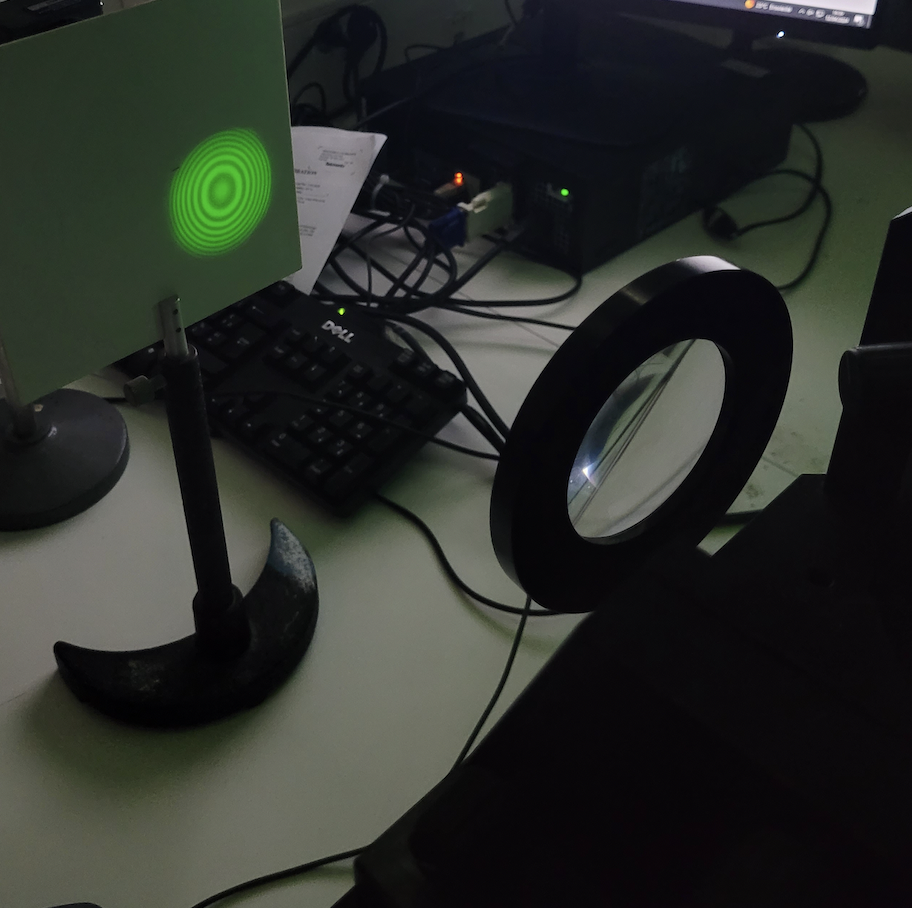
\includegraphics[height=5cm]{figs/anneaux.png}
            \caption{}\label{fig:anneaux}
        \end{subfigure}
    \end{subfigure}
    \caption{(\textbf{a}) Photo des deux images de croix superposées. On note les fines franges 
    d'interférences ressemblant à une empreinte digitale. (\textbf{b}) Système de franges circulaires projeté sur un écran à l'aide d'une lentille.}
\end{figure}

En mettant l'œil à la sortie de l'interféromètre, on voit une tache brilliante avec deux images de la croix - les miroirs n'étant pas parallèls, créent deux images indépendentes du même objet réel. On agit sur 
l'orientation de M1 ainsi que la position du condenseur pour superposer les deux images de croix. 
On voit alors des fines franges d'interférences, créant un motif ressemblant à une empreinte digitale (voir fig. \ref{fig:croix}).

On agit maintenant avec précaution sur les deux vis de réglages à l'arrière de M1 jusqu'à obtenir des anneaux concentriques 
centrés sur le champ d'observation. Nos deux miroirs sont alors à peu près parallèls.

Si les anneaux présentent un caractère elliptique, il se peut que la lame séparatrice ne soit pas bien réglé 
à 45°. Cela peut se vérifier en replaçant la source étendue par un laser pointé sur le miroir M2 et en 
vérifiant la lumière en sortie du Michelson avec un écran. Il faut absoluement éviter de regarder droit dans le faisceau laser, d'où 
l'utilisation de l'écran. Nous avons observé un multitude de points brilliants en sortie (plus que deux), ce qui est possiblement dû à des défauts visibles 
sur les miroirs. D'après ce que l'on à compris, afin de se rapprocher des 45°, il faut essayer de superposer aux mieux ces points lumineaux, 
en agissant sur l'angle d'incinaison de la lame séparatrice.

Nous remplaçons ensuite l'écran diffusant par un filtre vert afin d'isoler la raie d'émission à $546 \,\unit{nm}$ du Hg. 
Les interférences étant localisées à l'infini, nous plaçons une lentille convergente de focale $f = 20.0 \pm 0.5 \,\unit{cm}$ en sortie pour les projeter 
sur un écran. On place l'écran dans le plan focal image de manière approximative en maximisant la netteté et le contraste des anneaux (voir \ref{fig:anneaux}).

\subsection{Mesures expérimentales}

Les données analysées dans cette partie sont celles collectées par Théa Beaury et Yemen Cattabeni.

% Un fois l'interféromètre réglé, on trouve la position du miroir M1 correspondant à la teinte plate.
% À la teinte plate, les deux bras de l'inféromètres on exactement la même longeur, créant une illumination 
% uniforme de l'écran. Pour measurer la position de la teinte plate on observe la variation du rayons des anneaux 
% d'interférences. Lorsqu'on s'approche du contact optique (et donc de la teinte plate), le rayon des anneaux diminue 
% créant l'impression que les anneaux "rentrent" vers le centre. À l'inverse, lorsqu'on s'éloigne du contact optique, 
% le rayon des anneaux augmente, créant l'impression que les anneaux "sortent" du centre. 

Un fois l'interféromètre réglé, nous avons measuré la position de la teinte plate à l'œil nu après avec remplacé le filtre vert par l'écran diffusant.
On fait varier la position du miroir afin d'observer des anneaux "rentrants", et on continue jusqu'à ce qu'on observe une inversion 
dans le sens de déplacement des anneaux - indiquant qu'on est passé par la teinte plate. En passant à travers ce point d'inversion
à plusieurs reprises, on est donc capable de déduire la position approximative $x_0$ de la teinte plate. La position measurée par Théa et Yemen
est de $x_0 = 4.8 \pm 0.1 \,\textrm{mm}$.


%en variant continuellemnt la position du miroir 
%on measure la position de la teinte plate en variant continuellemnt la position du 
%miroir afin d'observer des anneaux "rentrant" jusqu'à ce qu'on observe une inversion dans le sens des 
%anneaux, indiquant qu'on est passé par la teinte plate. En passant à travers ce point d'inversion à plusieurs 
%reprises de façon de plus en plus minutieuse, on trouve la position approximative de la teinte plate à .
%Cette étape à été effectué à l'œil nu, 



Ensuite, on s'éloigne de la teinte plate jusqu'à observer un figure d'interférences avec au moins 10 anneaux brilliants.
Puis on remplace l'écran avec une barrette de photodiodes (caméra Caliens) en prenant soin de placer 
les photodiodes (et non le filtre assombrissant placé devant) dans le plan focal image de la lentille L. Une fois dans le plan focal image, 
on s'assure aussi de régler la position latérale de la caméra afin qu'elle coupe les anneaux en leur centre, 
nous permettant ainsi de mesurer le diamètre de chaques anneaux successifs. 

Avant de prendre des mesures, il faut impérativement noter la position du miroir M1 $x$. Cette information est nécessaire 
pour l'analyse des données plus tard. Dans le cas de Théa et de Yemen, la position mesurée était de $x=2.920 \pm 0.005 \,\textrm{mm}$, ce qui correspond à un déplacement absolu de 
$e = 1.9 \pm 0.1 \,\textrm{mm}$ du miroir mobile par rapport au contact optique.

Avec le logiciel Caliens, nous avons exporté les données contenant l'intensité mesurée par la caméra en fonction de la position verticale. En traçant ces données sur une figure, nous voyons des maxima correspondant au circonférences des anneaux d'interférences.

\begin{figure}[H]
    \centering
    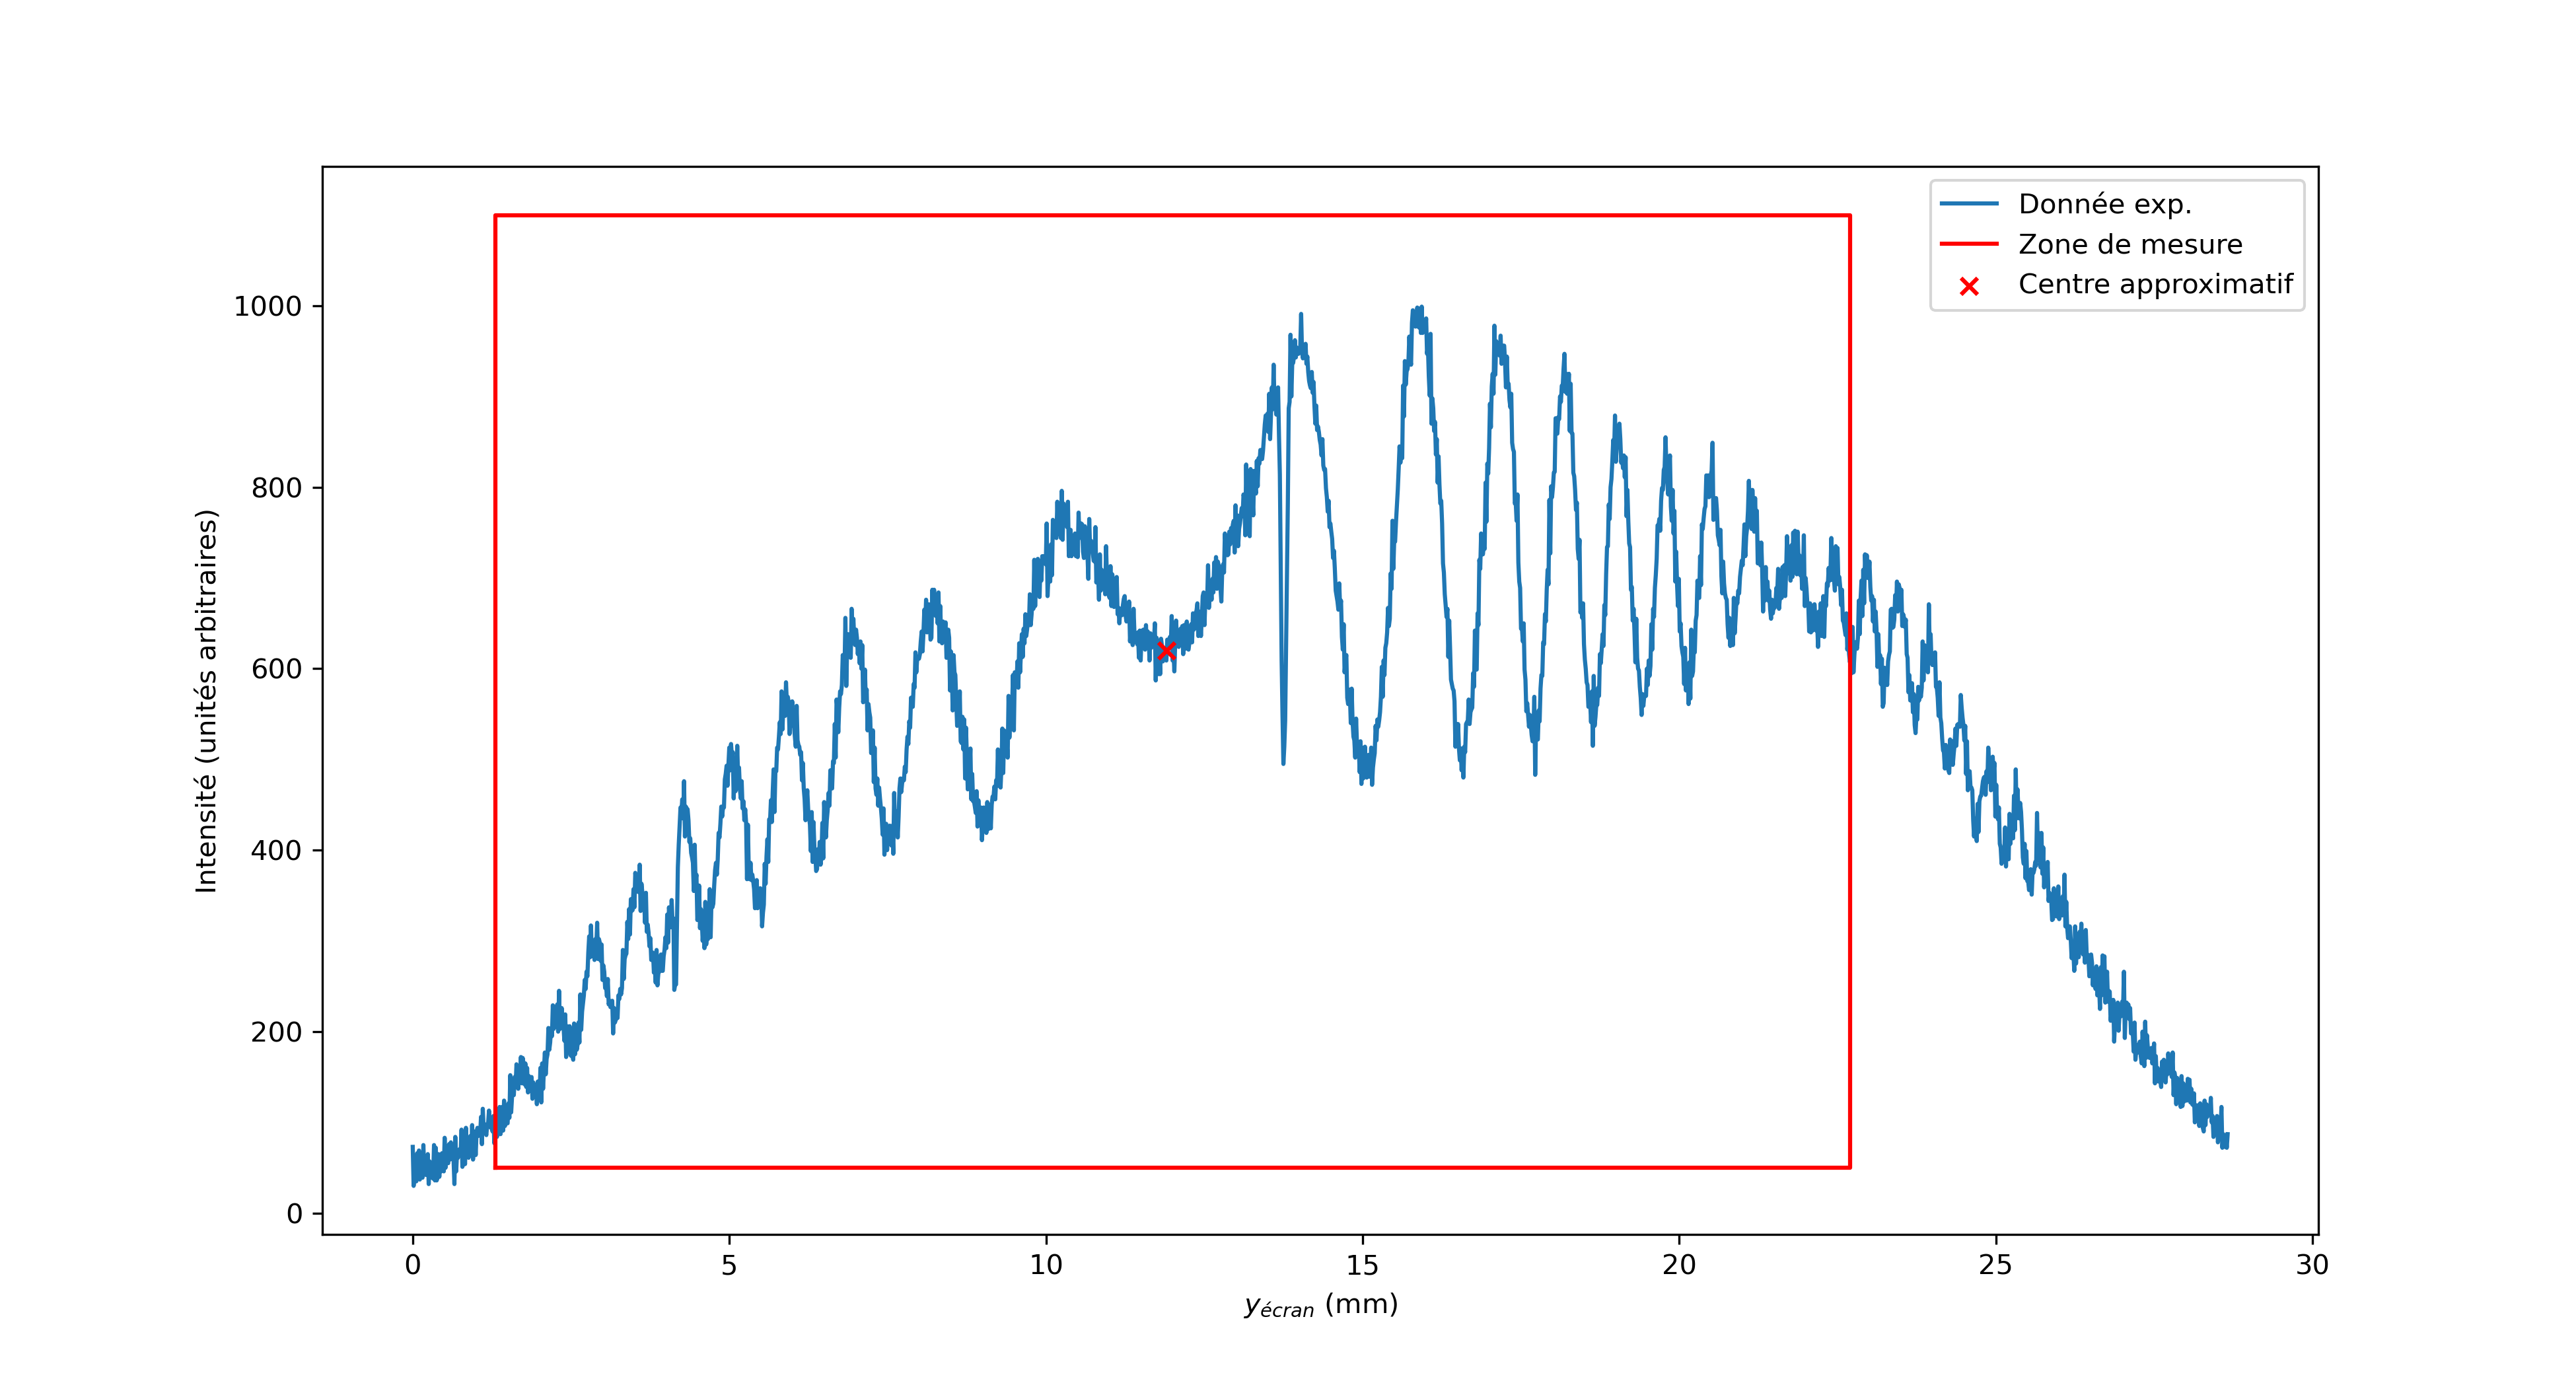
\includegraphics[width=0.8\linewidth]{figs/intensity_plt2.png}
    \caption{Tracé de l'intensité en fonction de la position verticale $y$ le long de la barrette de photodiodes. 
    On marque aussi la position approximative du centre de la figure d'interférences (croix rouge), 
    ainsi que la zone contenant les dix premiers anneaux (rectange rouge).}
    \label{fig:diff_1}
\end{figure}

Pour chaques anneaux, on repère les deux maxima lui correspondant en partant du centre de la figure d'interférences. 
On obtient le diamètre en calculant la distance séparant les deux maximas. 
Le bruit sur la figure rendant la mesure de la position des maxima assez inexacte, on prend une 
incertitude de mesure de 0.2 mm par maximum. Pour l'incertitude du diamètre, les intertitudes 
sur les positions des deux maxima s'ajoutent en quadrature pour donner 
$\Delta D_q \approx 0.3 \,\textrm{mm}$. 

On repète cette même procédure pour les dix prémiers anneaux en partant du centre.


\subsection{Analyse et Interprétations}

On peut montrer que le rayon $R_q$ du $q$-ième anneau brillant formé dans le plan focal image
de la lentille L (distance focale $f$) est donné par :

\begin{equation}
    R_q = f \sqrt{\frac{\lambda}{e}(q-1+\epsilon)}
\end{equation}

Ce qui implique la relation suivante pour le diamètre carré $D_q^2$ du $q$-ième anneau :

\begin{equation}
    D_q^2 = f^2 \frac{\lambda}{e}(q-1+\epsilon)
    \label{eq:dq2}
\end{equation}

La relation liant $D_q^2$ et $q$ est donc affine, avec une pente théorique de $ \frac{f^2 \lambda}{e} = (4.72\pm0.35)\times10^{-6} \,\textrm{m}^2$.
On vérifie cela en traçant les valeurs experimentales de $D_q^2$ en fonction de $q$.

\begin{figure}[H]
    \centering
    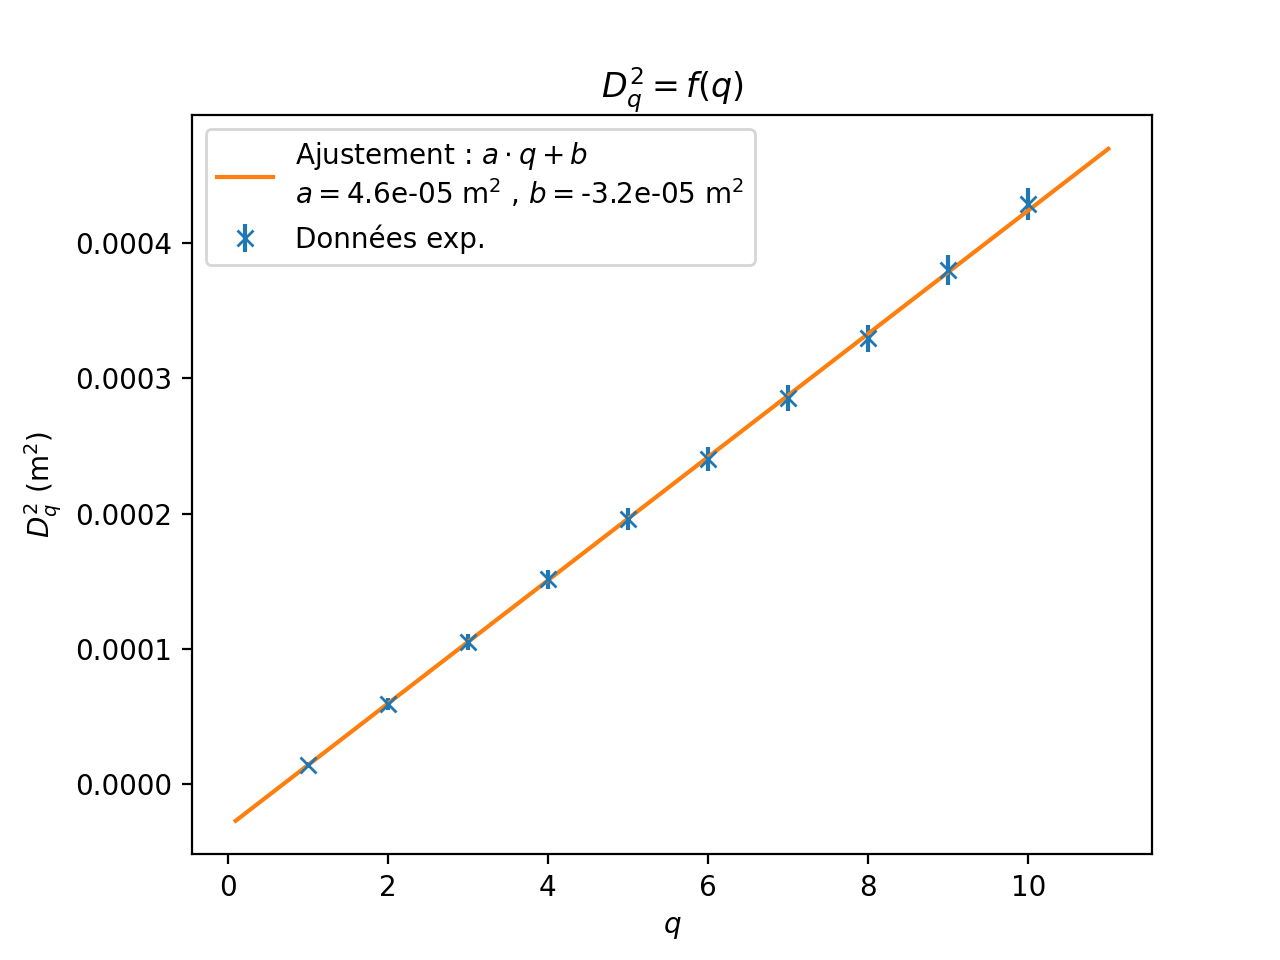
\includegraphics[width=0.6\linewidth]{figs/D2_q.png}
    \caption{Traçé de $D_q^2$ en fonction de $q$ avec un ajustement affine $D_q^2=a\cdot q+b$ avec pour paramètres 
    $a=(4.56\pm0.02)\times10^{-5} \,\textrm{m}^2$ et $b = (-3.16 \pm 0.05) \times 10^{-5} \,\textrm{m}^2$.}
\end{figure}

La pente de la courbe adjustée $a=(4.56\pm0.02)\times10^{-5} \,\textrm{m}^2$ est bien en concordance avec la valeur théorique. 
La lumière étant monochromatique avec $\lambda = 546 \,\unit{nm}$, on est capable d'en déduire la valeur de l'excédent fractionnel $\epsilon$ à partir de 
\eqref{eq:dq2} et de la valeur de $b$. On doit nécessairement obtenir une valeur entre 0 et 1.

$$ b = f^2 \frac{\lambda}{e}(\epsilon - 1) \implies \epsilon = 0.33 \pm 0.08$$

D'après le tracé d'intensité fig. \ref{fig:diff_1}, le premier anneau brilliant n'est pas précédé par un anneau sombre.
Donc la valeur experimentale $\epsilon = 0.33 \pm 0.08$ est bien cohérente avec les observations. 
En effet, lorsque le premier anneau brilliant est précédé par un anneau sombre d'ordre supérieur on devrait avoir $\epsilon > 0.5$, et dans le cas contraire
 $\epsilon < 0.5$. 


\newpage

\section{Mesure de l'écart du doublet du sodium}

Le but de cette manipulation est de déterminer à l’aide d’un interféromètre de Michelson 
l’écart de longueur d’onde $\Delta \lambda$ du doublet du sodium en trouvant les épaisseurs de lame d’air 
auxquelles on observe un brouillage.

Le spectre d'émission du sodium comporte deux raies d'émission de longeurs d'onde $\lambda_1$, $\lambda_2$ très proches.
La longeur d'onde moyenne de ce doublet est $\lambda_m = 589 \,\unit{nm}$ et nous cherchons l'écart $\Delta \lambda$ entre ces deux raies 
défini tel que $\lambda_2 = \lambda_1 + \Delta \lambda$.

Chacunes de ces deux radiations crée sont propre système d'intérférences qui se superposent de manière 
incohérente. En s'appuyant sur le fait que $\lambda_m \gg \Delta \lambda$, et en considérant que les intensité lumineuses
 des deux raies sont les mêmes, on trouve l'intensité totale en un point $M$ en sortie du Michelson :

\begin{equation}
I(M)=I_0 \cdot\left[1+\cos \left(\pi \frac{\delta}{\lambda_m^2 / \Delta \lambda}\right) \cos \left(2 \pi \frac{\delta}{\lambda_m}\right)\right]
\end{equation}

À des positions particulières $x$ du miroir mobile, les minima d'un des systèmes de franges se superposent sur les maximas de l'autre, 
brouillant la figure d'interférences. On rend compte de ce phénomène avec le terme $\cos \left(\pi \frac{\delta}{\lambda_m^2 / \Delta \lambda}\right)$ 
dont la période en fonction de $\delta$ est $\frac{\lambda_m^2}{2\Delta \lambda}$. Donc la variation de la différence de marche $\Delta \delta$ entre deux positions de brouillages consécutifs est la suivante :

$$\Delta \delta = \frac{\lambda_m^2}{\Delta \lambda}$$

Vu à un angle d'incidence $\theta$, la différence de marche est $\delta = 2e\cos(\theta)$, avec $e$ l'épaisseur de la lame d'air. 
Pour de petits $\theta$, nous prenons comme première approximation $\delta = 2e$. Donc entre deux brouillages, le mirroir mobile doit se déplacer de 
$\Delta x = \frac{\lambda_m^2}{2\Delta \lambda}$ (on rappelle que $e = x - x_0$). On déduit $\Delta \lambda$ en mesurant $\Delta x$ :

\begin{equation}
    \Delta \lambda = \frac{\lambda_m^2}{2\Delta x}
    \label{eq:deltalambda}
\end{equation}

\par 
\par 

\begin{figure}[H]
    \centering
    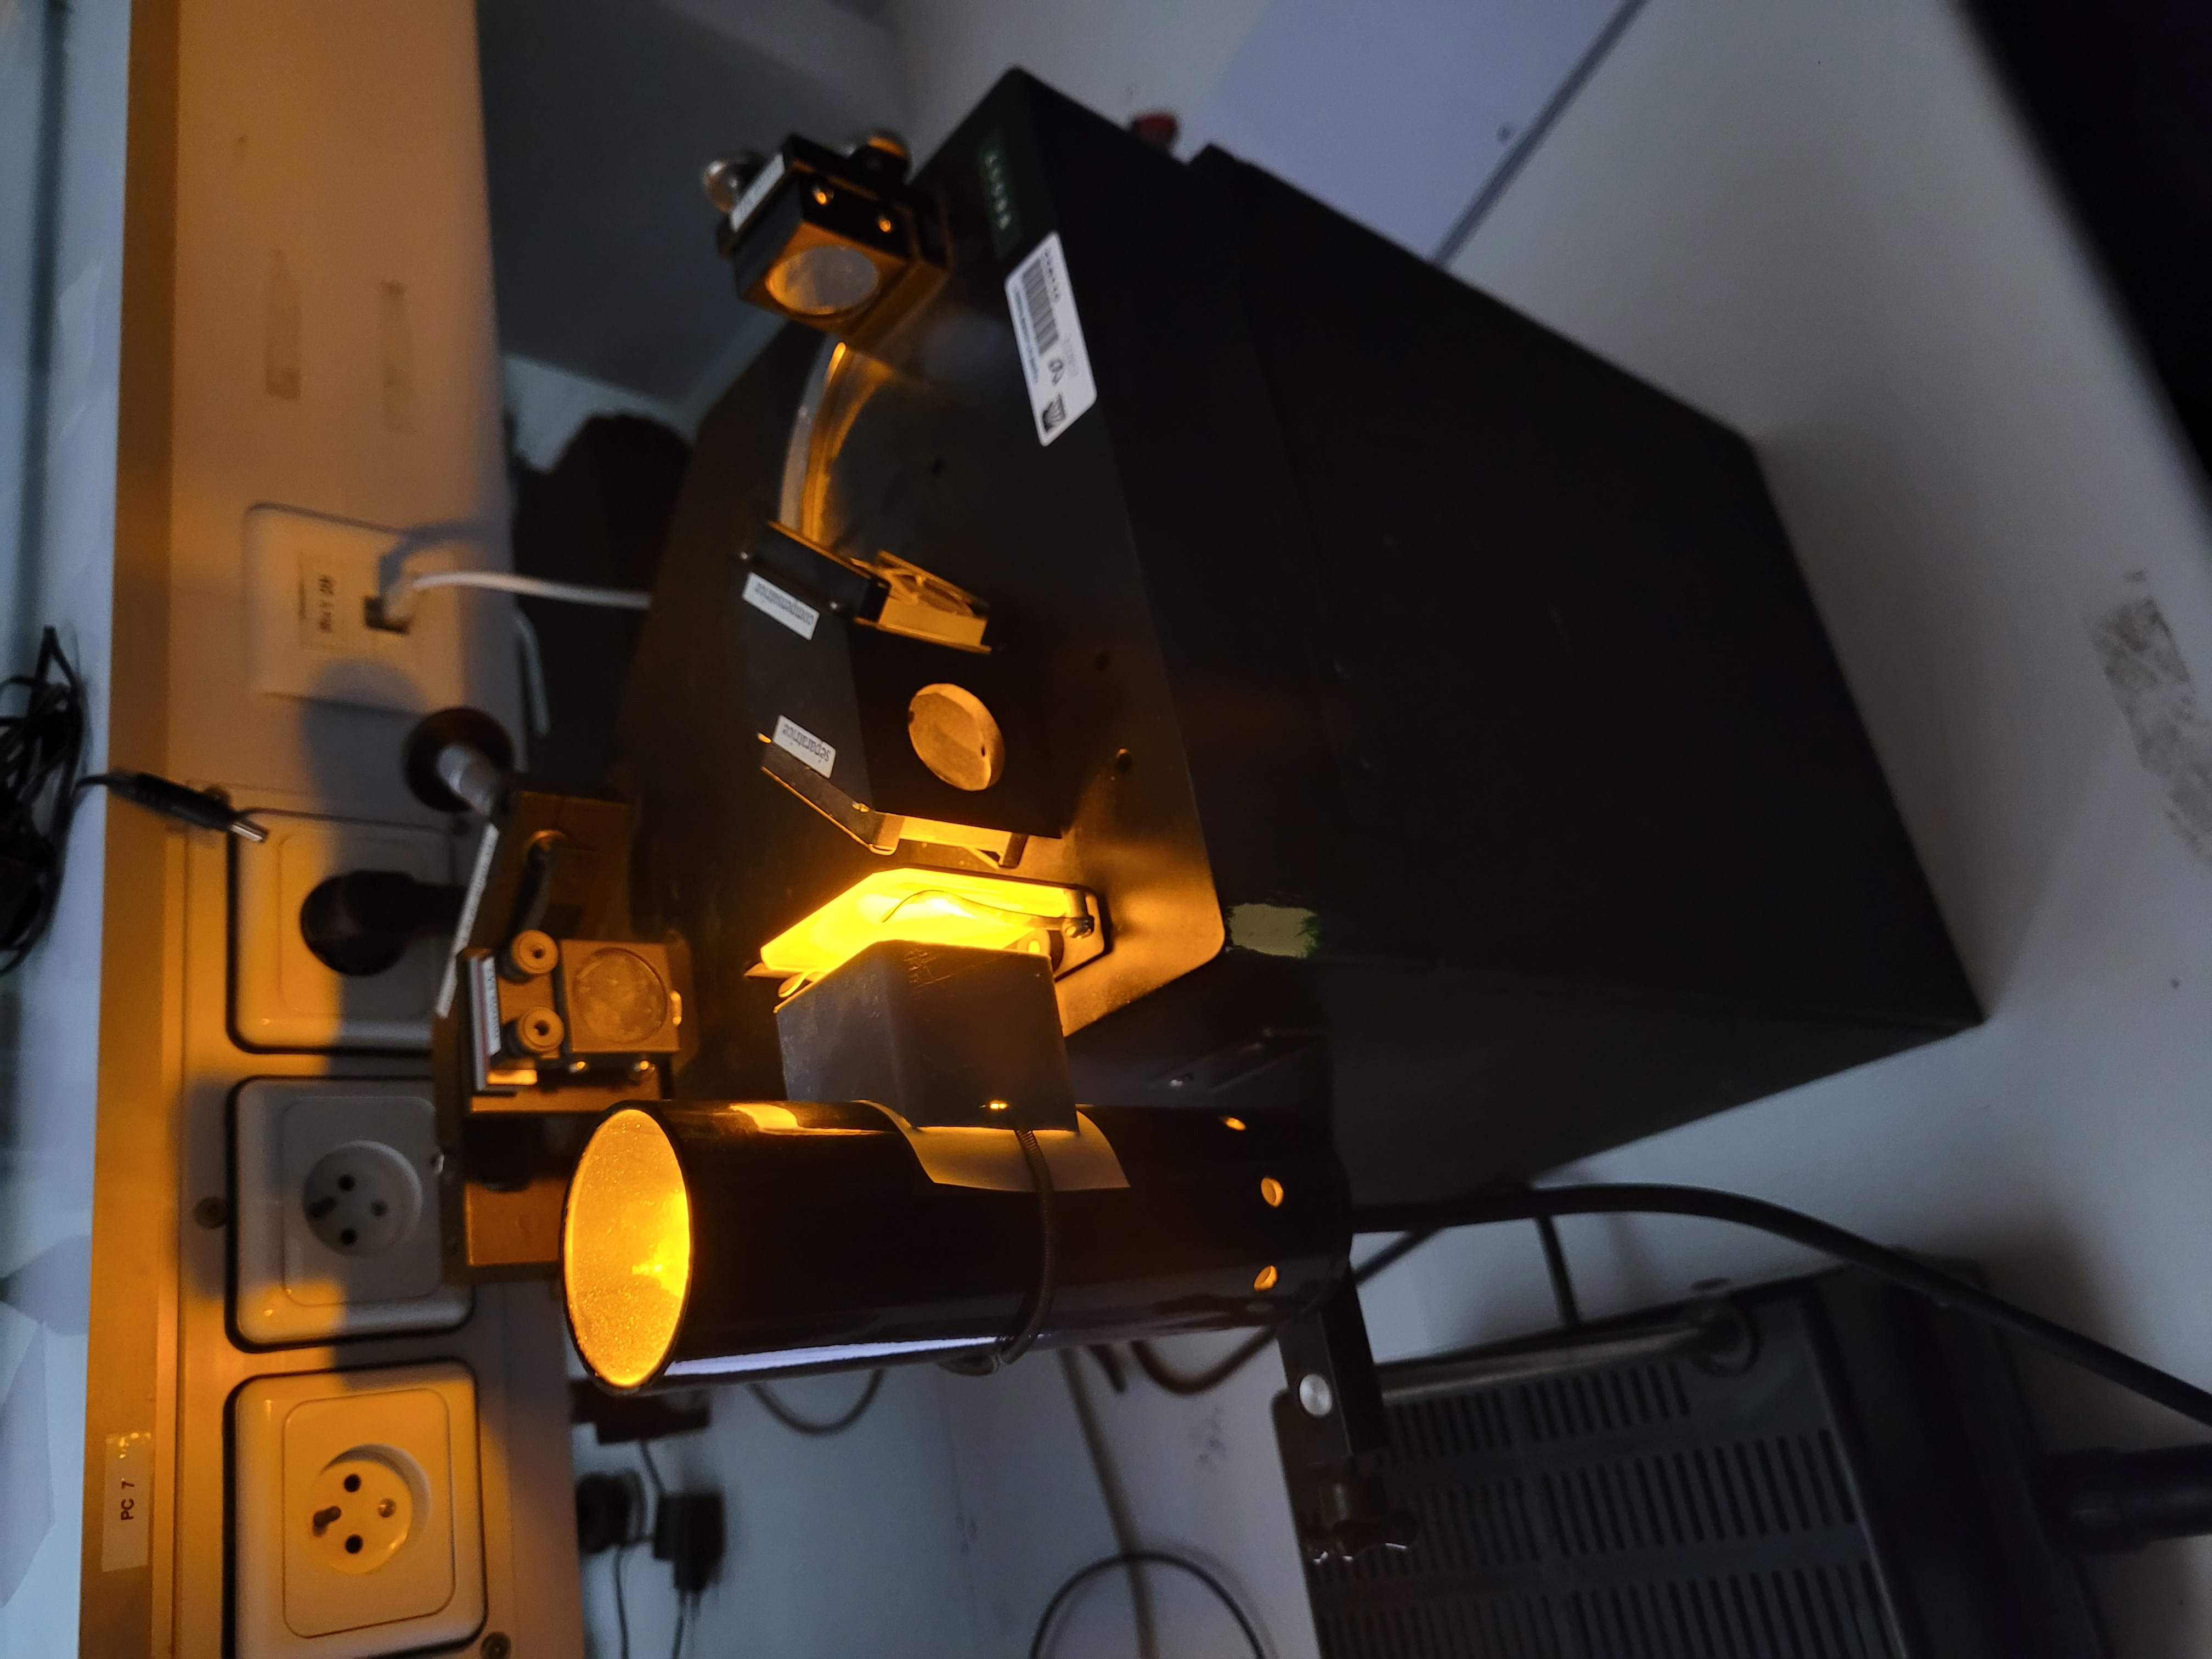
\includegraphics[angle=-90, width=0.4\linewidth]{figs/sodium.jpg}
    \caption{Photo de l'interféromètre éclairé par la lampe à sodium}
    \label{fig:michelson}
\end{figure}

\newpage
\subsection{Mesures expérimentales}

Les mesures se font encore une fois en configuration lame d'air. L'interféromètre était déjà réglé à 
notre arrivée, mais sinon les réglages auraient été les mêmes que pour la manipulation précédente.

On commence par mesurer les positions du mirroir mobile $x$ auxquelles on observe un brouillage. 
Dans notre cas, nous avons observé que la principale source d'erreur dans ces mesures provenait de la difficulté 
à déterminer la position éxacte d'un brouillage à l'œil, l'incertitude intrinsèque du vernier est négligeable par rapport à cette erreur. 
Pour chaque brouillage, nous avons donc mesuré les deux positions extrêmes $x_{\textrm{min}}$, $x_{\textrm{max}}$ entre lesquelles on observe un brouillage. 
Ensuite on obtient la valeur expérimentale pour chaque position de brouillage $x_i$ et son incertitude $\Delta (x_i)$ avec les formules 
suivantes :

\begin{equation}
    x_i = \frac{x_{\textrm{max}} + x_{\textrm{min}}}{2} \qquad \Delta(x_i) = x_{\textrm{max}} - x_i
\end{equation}

\begin{table}[H]
\begin{center}
    \begin{tabular}{|c|c|c|c|c|}
        \hline 
        brouillage $i$ & $x_{i\textrm{, min}}$ (mm) & $x_{i\textrm{, max}}$ (mm) & $x_{i}$ (mm) & $\Delta(x_i)$ (mm)\\
        \hline 
        1 & 10.640 & 10.695 & 10.67 & 0.03 \\
        \hline 
        2 & 12.100 & 12.150 & 12.13 & 0.03 \\
        \hline 
        3 & 13.540 & 13.555 & 13.548 & 0.008 \\
        \hline 
        4 & 15.020 & 15.045 & 15.03 & 0.02 \\
        \hline 
        5 & 16.470 & 16.510 & 16.49 & 0.02 \\
        \hline 
        6 & 17.895 & 17.960 & 17.93 & 0.04 \\
        \hline 
        7 & 19.380 & 19.420 & 19.40 & 0.02 \\
        \hline
    \end{tabular}
    \caption{Mesures des positions de brouillage}
\end{center}
\end{table}

\subsection{Détermination de $\Delta \lambda$}

Nous calculons ensuite l'écart entre les positions de brouillage consécutives $\Delta x_{i, j}$, ainsi que son incertitude en ajoutant les incertitudes 
des deux positions en quadrature.

\begin{equation}
    \Delta x_{i, j} = |x_i - x_j| \qquad \Delta(\Delta x_{i, j}) = \sqrt{(\Delta(x_i))^2 + (\Delta(x_j))^2}
\end{equation}

\begin{table}[H]
\begin{center}
    \begin{tabular}{|c|c|c|}
        \hline $i, j$ & $\Delta x_{i, j}$ (mm) & $\Delta(\Delta x_{i, j})$ (mm) \\
        \hline 1,2 & 1.46 & 0.05 \\
        \hline 2,3 & 1.42 & 0.04 \\
        \hline 3,4 & 1.48 & 0.03 \\
        \hline 4,5 & 1.46 & 0.03 \\
        \hline 5,6 & 1.44 & 0.05 \\
        \hline 6,7 & 1.47 & 0.05 \\
        \hline
    \end{tabular}
    \caption{Écarts entre positions de brouillage}
\end{center}
\end{table}

Nous obtenons des écarts très similaires, ce qui est rassurant, et on calcule un écart moyen $\Delta x = 1.46 \pm 0.05 \,\unit{mm}$. 

En utilisant la relation théorique \eqref{eq:deltalambda}, on obtient $\Delta \lambda = 1.22 \pm 0.05 \,\unit{\angstrom}$. 
Or, d'àpres \href{https://fr.wikipedia.org/wiki/Doublet_du_sodium}{Wikipedia}, 
l'écart réel est cinq fois plus grand $\Delta \lambda_{\textrm{réel}} = 5.974 \,\unit{\angstrom}$.

Visiblement, quelque chose n'est pas correct. Il est possible que nous ayons systèmatiquement raté des positions de brouillages entre 
celles qui ont été mesurées, ce qui aurait conduit à une surevaluation de $\Delta x$. 
Or l'absence de valeurs aberrantes des nos mesures ne soutient pas cette affirmation, et il est peu probable que l'erreur humaine ait pu 
être aussi systèmatique.

Malgré cela, cette mesure est quand même au bon ordre de grandeur. Et le fait qu'on ai pu mesurer une différence de l'ordre de l'angstrom, 
c'est à dire l'ordre de grandeur de la taille d'un atome, est tout de même très impressionant!


\section{Conclusion}

% À travers ces deux expériences, nous avons appris à regler un interféromètre de Michelson en configuration "lame d'air" 
% ainsi qu'interpeter la figure d'interférences pour déduire des propriétés de notre système.

% L'interférometre est un instrument de mesure extremement sensible, chose que nous avons pu observer lors de nos manipulations. 
% Chaque ajustement, même minime, de la disposition de l'appareil ou de la table expérimentale entraînait des variations significatives 
% dans la figure d'interférence observée.

En conclusion, nos expériences avec l'interféromètre de Michelson ont permis d'atteindre plusieurs objectifs. 
Nous avons réussi à régler l'interféromètre en configuration "lame d'air" et à observer des figures d'interférences claires et nettes, 
confirmant ainsi le bon fonctionnement de l'appareil. De plus, nous avons réalisé des mesures de l'écart du doublet du sodium, 
bien que la valeur expérimentale obtenue soit inférieure à la valeur attendue.

Nos résultats soulignent la sensibilité et la précision de l'interféromètre de Michelson en tant qu'outil de mesure des différences de longueur 
d'onde. Les applications de cet instrument vont au-delà de la simple détermination des écarts spectraux, et il peut être utilisé dans de nombreux 
domaines, tels que la spectroscopie, la métrologie, et même la détection des ondes gravitationnelles.

Nous avons appris des leçons importantes lors de ces manipulations, en particulier l'importance de toujours bien documenter 
ses mesures afin d'éviter la perte de données. Pour des travaux futurs, il serait intéressant d'explorer d'autres configurations de l'interféromètre de Michelson, 
en particulier la configuration coin d'air. 
Il serait aussi souhaitable de reprendre les mesures sur le doublet du sodium pour determiner la source de nos résultats erronés.


\end{document}